\documentclass[14pt]{extbook}
\usepackage{multicol, enumerate, enumitem, hyperref, color, soul, setspace, parskip, fancyhdr} %General Packages
\usepackage{amssymb, amsthm, amsmath, bbm, latexsym, units, mathtools} %Math Packages
\everymath{\displaystyle} %All math in Display Style
% Packages with additional options
\usepackage[headsep=0.5cm,headheight=12pt, left=1 in,right= 1 in,top= 1 in,bottom= 1 in]{geometry}
\usepackage[usenames,dvipsnames]{xcolor}
\usepackage{dashrule}  % Package to use the command below to create lines between items
\newcommand{\litem}[1]{\item#1\hspace*{-1cm}\rule{\textwidth}{0.4pt}}
\pagestyle{fancy}
\lhead{Makeup Progress Quiz 1}
\chead{}
\rhead{Version B}
\lfoot{6018-3080}
\cfoot{}
\rfoot{Spring 2021}
\begin{document}

\begin{enumerate}
\litem{
Determine the domain of the function below.\[ f(x) = \frac{4}{12x^{2} -34 x + 24} \]\begin{enumerate}[label=\Alph*.]
\item \( \text{All Real numbers except } x = a \text{ and } x = b, \text{ where } a \in [11.86, 12.1] \text{ and } b \in [23.71, 24.01] \)
\item \( \text{All Real numbers.} \)
\item \( \text{All Real numbers except } x = a, \text{ where } a \in [1.07, 1.38] \)
\item \( \text{All Real numbers except } x = a \text{ and } x = b, \text{ where } a \in [1.07, 1.38] \text{ and } b \in [1.41, 1.58] \)
\item \( \text{All Real numbers except } x = a, \text{ where } a \in [11.86, 12.1] \)

\end{enumerate} }
\litem{
Solve the rational equation below. Then, choose the interval(s) that the solution(s) belongs to.\[ \frac{7x}{3x -2} + \frac{-2x^{2}}{-21x^{2} -x + 10} = \frac{5}{-7x -5} \]\begin{enumerate}[label=\Alph*.]
\item \( x_1 \in [0.12, 0.44] \text{ and } x_2 \in [-3.15,-0.15] \)
\item \( x \in [-0.88,-0.65] \)
\item \( x_1 \in [0.12, 0.44] \text{ and } x_2 \in [-0.33,4.67] \)
\item \( \text{All solutions lead to invalid or complex values in the equation.} \)
\item \( x \in [-1.37,-1.07] \)

\end{enumerate} }
\litem{
Choose the graph of the equation below.\[ f(x) = \frac{1}{(x - 3)^2} - 2 \]\begin{enumerate}[label=\Alph*.]
\begin{multicols}{2}\item 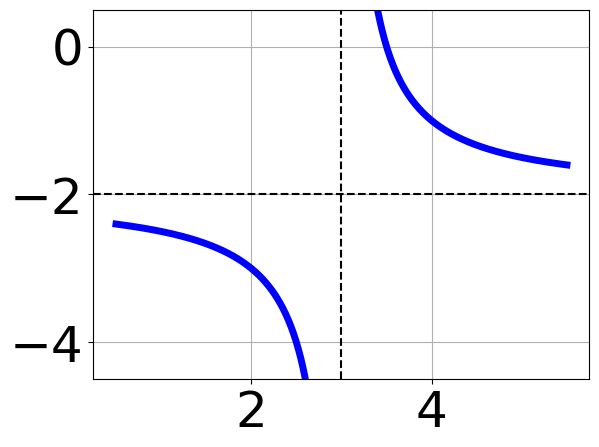
\includegraphics[width = 0.3\textwidth]{../Figures/rationalEquationToGraphCopyAB.png}\item 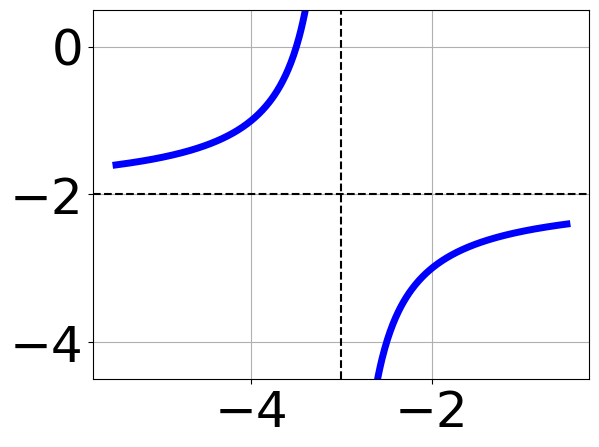
\includegraphics[width = 0.3\textwidth]{../Figures/rationalEquationToGraphCopyBB.png}\item 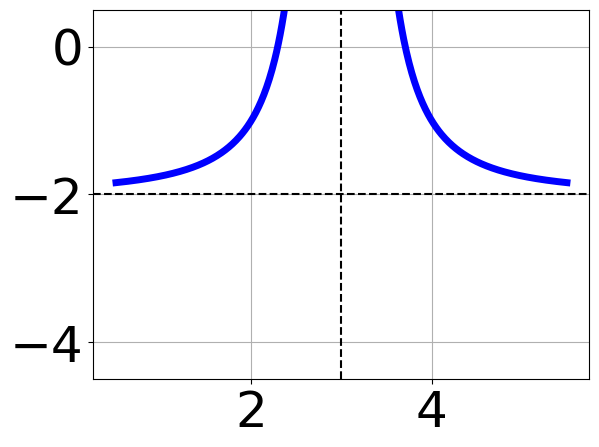
\includegraphics[width = 0.3\textwidth]{../Figures/rationalEquationToGraphCopyCB.png}\item 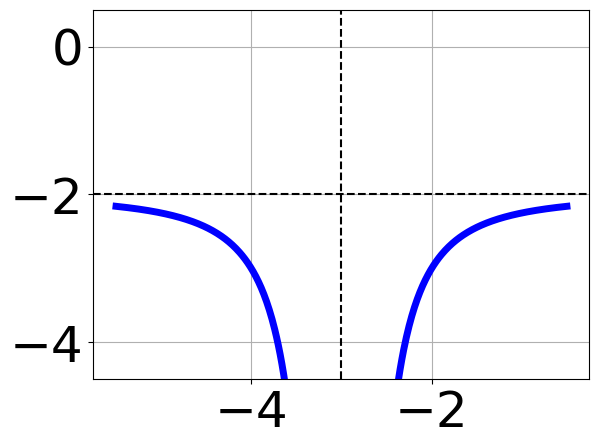
\includegraphics[width = 0.3\textwidth]{../Figures/rationalEquationToGraphCopyDB.png}\end{multicols}\item None of the above.
\end{enumerate} }
\litem{
Choose the graph of the equation below.\[ f(x) = \frac{1}{(x - 3)^2} - 1 \]\begin{enumerate}[label=\Alph*.]
\begin{multicols}{2}\item 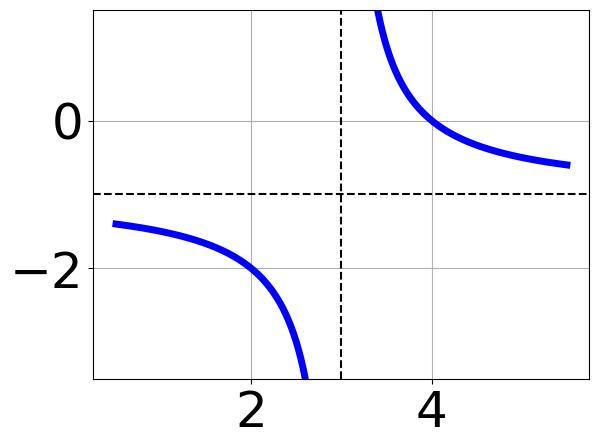
\includegraphics[width = 0.3\textwidth]{../Figures/rationalEquationToGraphAB.png}\item 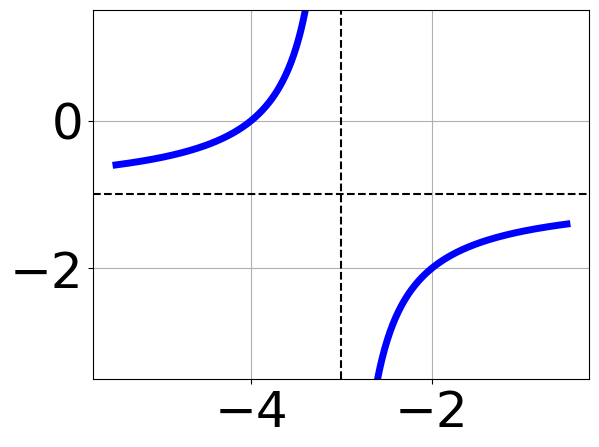
\includegraphics[width = 0.3\textwidth]{../Figures/rationalEquationToGraphBB.png}\item 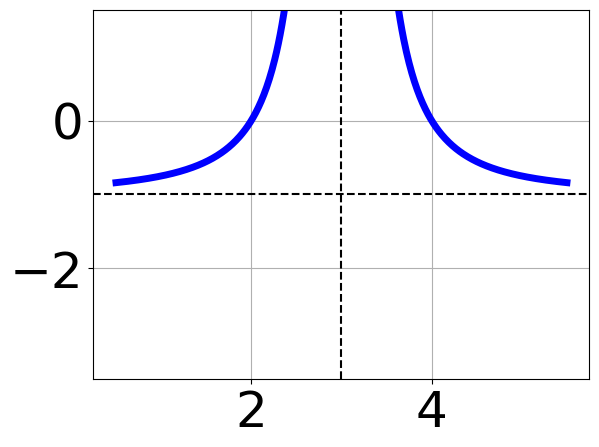
\includegraphics[width = 0.3\textwidth]{../Figures/rationalEquationToGraphCB.png}\item 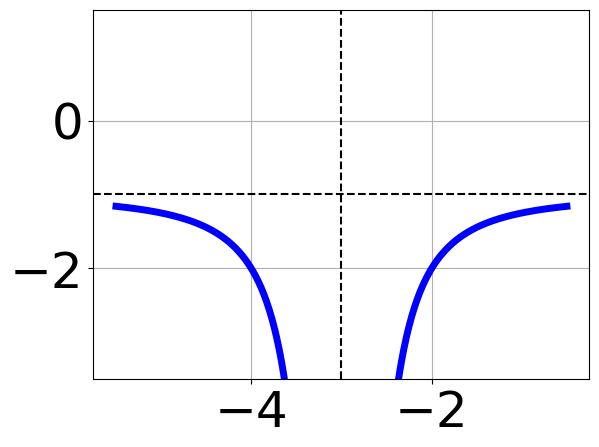
\includegraphics[width = 0.3\textwidth]{../Figures/rationalEquationToGraphDB.png}\end{multicols}\item None of the above.
\end{enumerate} }
\litem{
Choose the equation of the function graphed below.
\begin{center}
    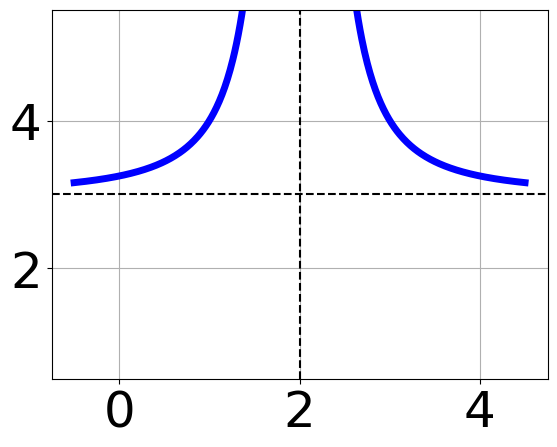
\includegraphics[width=0.5\textwidth]{../Figures/rationalGraphToEquationCopyB.png}
\end{center}
\begin{enumerate}[label=\Alph*.]
\item \( f(x) = \frac{-1}{x - 2} + 3 \)
\item \( f(x) = \frac{1}{x + 2} + 3 \)
\item \( f(x) = \frac{-1}{(x - 2)^2} + 3 \)
\item \( f(x) = \frac{1}{(x + 2)^2} + 3 \)
\item \( \text{None of the above} \)

\end{enumerate} }
\litem{
Solve the rational equation below. Then, choose the interval(s) that the solution(s) belongs to.\[ \frac{3x}{5x + 6} + \frac{-5x^{2}}{10x^{2} +22 x + 12} = \frac{-4}{2x + 2} \]\begin{enumerate}[label=\Alph*.]
\item \( x_1 \in [-25.06, -25.02] \text{ and } x_2 \in [-1.2,-1.19] \)
\item \( x_1 \in [-25.06, -25.02] \text{ and } x_2 \in [-1,-0.85] \)
\item \( x \in [-1.02,-0.97] \)
\item \( x \in [-0.99,-0.93] \)
\item \( \text{All solutions lead to invalid or complex values in the equation.} \)

\end{enumerate} }
\litem{
Determine the domain of the function below.\[ f(x) = \frac{4}{12x^{2} -36 x + 24} \]\begin{enumerate}[label=\Alph*.]
\item \( \text{All Real numbers except } x = a \text{ and } x = b, \text{ where } a \in [0.8, 1.4] \text{ and } b \in [1.7, 2.6] \)
\item \( \text{All Real numbers except } x = a, \text{ where } a \in [15.7, 17] \)
\item \( \text{All Real numbers.} \)
\item \( \text{All Real numbers except } x = a \text{ and } x = b, \text{ where } a \in [15.7, 17] \text{ and } b \in [16.3, 19.5] \)
\item \( \text{All Real numbers except } x = a, \text{ where } a \in [0.8, 1.4] \)

\end{enumerate} }
\litem{
Choose the equation of the function graphed below.
\begin{center}
    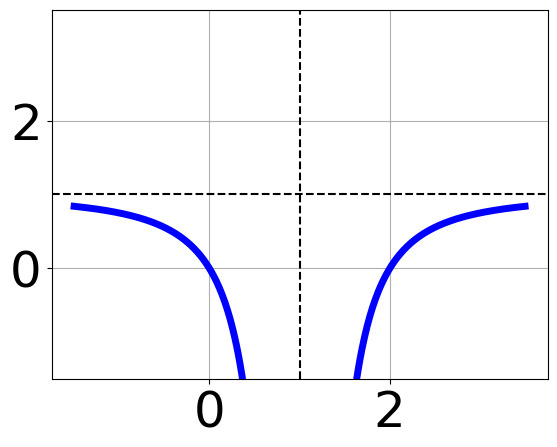
\includegraphics[width=0.5\textwidth]{../Figures/rationalGraphToEquationB.png}
\end{center}
\begin{enumerate}[label=\Alph*.]
\item \( f(x) = \frac{1}{x + 1} + 1 \)
\item \( f(x) = \frac{-1}{x - 1} + 1 \)
\item \( f(x) = \frac{1}{(x + 1)^2} + 1 \)
\item \( f(x) = \frac{-1}{(x - 1)^2} + 1 \)
\item \( \text{None of the above} \)

\end{enumerate} }
\litem{
Solve the rational equation below. Then, choose the interval(s) that the solution(s) belongs to.\[ \frac{-3}{5x + 4} + 4 = \frac{-6}{15x + 12} \]\begin{enumerate}[label=\Alph*.]
\item \( x_1 \in [-0.85, -0.71] \text{ and } x_2 \in [0.85,2.85] \)
\item \( \text{All solutions lead to invalid or complex values in the equation.} \)
\item \( x \in [0.75,1.05] \)
\item \( x_1 \in [-0.97, -0.78] \text{ and } x_2 \in [-1.75,0.25] \)
\item \( x \in [-0.75,0.25] \)

\end{enumerate} }
\litem{
Solve the rational equation below. Then, choose the interval(s) that the solution(s) belongs to.\[ \frac{18}{18x + 81} + 1 = \frac{18}{18x + 81} \]\begin{enumerate}[label=\Alph*.]
\item \( x_1 \in [-5.5, -3.5] \text{ and } x_2 \in [-5.5,-3.5] \)
\item \( x \in [-4.5,-2.5] \)
\item \( x \in [4.5,6.5] \)
\item \( x_1 \in [-5.5, -3.5] \text{ and } x_2 \in [4.5,6.5] \)
\item \( \text{All solutions lead to invalid or complex values in the equation.} \)

\end{enumerate} }
\end{enumerate}

\end{document}